\documentclass[10pt,twocolumn]{report}
\usepackage{ctex}
\usepackage[utf8]{inputenc}
\usepackage{amsmath}
\usepackage{amssymb}
\usepackage{xcolor}
\usepackage{graphicx}
\usepackage[margin=0.1cm]{geometry} % 设置页边距为 0.5cm，尽可能扩大可用区域
\usepackage{setspace}
\renewcommand{\baselinestretch}{1} % 设置行间距为单倍行距
\usepackage{float}
\usepackage{wrapfig}
\usepackage[utf8]{inputenc}
\usepackage[T1]{fontenc}
\usepackage{ctex}
\usepackage{amsmath}
\usepackage{amssymb}
\usepackage{booktabs} 
\usepackage{xcolor}
\usepackage{graphicx}
\usepackage{float}
\usepackage{lmodern}
\usepackage{mathrsfs}
\usepackage{lipsum}
\usepackage{array} 
\usepackage{tikz}
\usepackage{braket}
\usepackage{adjustbox}
\usepackage{footmisc}
\usepackage{array}
\usepackage{multirow}
\usepackage[table]{xcolor}
\usepackage{amsmath}
\usepackage{tcolorbox}
\usepackage{caption}
\usepackage{tabularx}
\captionsetup[figure]{labelformat=empty} % 设置图标题的标签格式为空，即不显示“图 X”
\usepackage{graphicx}
\tcbuselibrary{listings,breakable}
\usepackage{xcolor}
\setlength{\parindent}{0pt}
\captionsetup[figure]{skip=0pt}
\usepackage{array}
\title{光纤}
\author{张世航}
\begin{document}
     \maketitle
     \section{表1}
     \begin{table}[H]
     	\centering
     	\setlength{\extrarowheight}{4pt}  
     	\resizebox{0.45\textwidth}{!}{
     \begin{tabular}{|c|c|c|c|c|c|c|c|c|c|c|}
     	\hline
     	发射电流($\times$ 10mA) & 0 & 0.5 & 0.6 & 0.8 & 1 & 1.5 & 2.0 & 2.5 & 3.0 & 3.5 \\
     	\hline
     	正向偏压(V) & 0.73 & 0.97 & 0.99 & 1.01 & 1.02 & 1.06 & 1.09 & 1.13 & 1.16 & 1.19 \\
     	\hline
     	光功率(mW) & -0.019 & -0.019 & -0.019 & -0.013 & 0.027 & 0.150 & 0.274 & 0.402 & 0.523 & 0.645 \\
     	\hline
     \end{tabular}
    }
    \end{table}
     \begin{figure}[H]
     	\centering
     	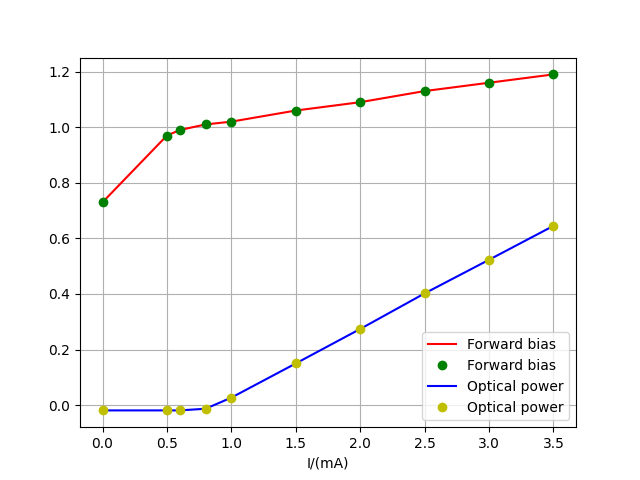
\includegraphics[width=0.7\linewidth]{picture_1}
     	\caption{表1}
     	\label{fig:picture1}
     \end{figure}
     \section{表2}
     \begin{tabular}{|c|c|c|c|c|c|}
     	\hline
     	反向偏置电压(V) & 0 & 1 & 2 & 3 & 4 \\
     	\hline
     	P=0 & 0 & 0 & 0 & 0 & 0 \\
     	\hline
     	P=0.1mW & 111 & 111 & 111 & 111 & 111 \\
     	\hline
     	P=0.2mW & 220 & 220 & 220 & 220 & 220 \\
     	\hline
     \end{tabular}
     \begin{figure}[H]
     	\centering
     	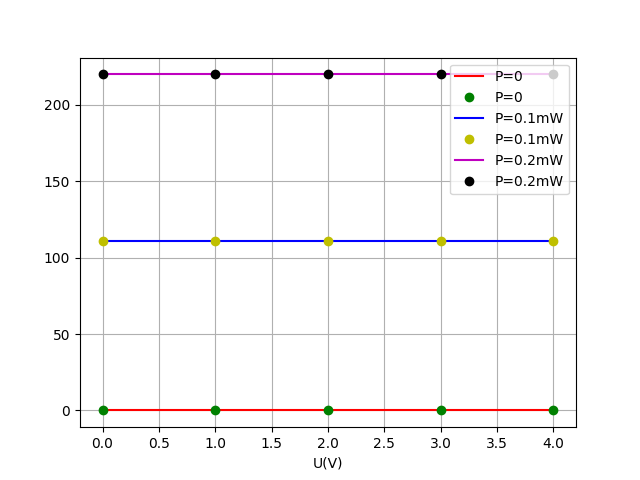
\includegraphics[width=0.7\linewidth]{picture_2}
     	\caption{}
     	\label{fig:picture2}
     \end{figure}
     
     \section{表3}
     \begin{tabular}{ccccc}
     	\toprule
     	& \multicolumn{2}{c}{激光二极管调制电路输入信号} & \multicolumn{2}{c}{光电二极管转换电路输出信号} \\
     	\cmidrule(lr){2-3} \cmidrule(lr){4-5}
     	波形 & 频率(kHz) & 幅度(V) & 频率(kHz) & 幅度(V) \\
     	\midrule
     	正弦波 & 5.0 & 2.03 & 5.0 & 0.488 \\
     	方波 & 5.0 & 2.07 & 5.0 & 0.496 \\
     	\bottomrule
     \end{tabular}
     
     \section{表4}
     \begin{table}[H]
     	\centering
     	\setlength{\extrarowheight}{4pt}  
     	\resizebox{0.45\textwidth}{!}{
     \begin{tabular}{|c|c|c|c|c|c|c|c|c|c|c|c|}
     	\hline
     	输出电压(V) & 0 & 0.5 & 1.0 & 1.5 & 2.0 & 2.5 & 3.0 & 3.5 & 4.0 & 4.5 & 5.0 \\
     	\hline
     	输出频率$f_v(kHz)$ &84.65& 82.46& 80.65 &78.01& 76.83 &73.96& 72.2&  69.28& 67.6 & 64.88 &62.74 \\
     	\hline
     	角频率$\omega(kHz)$ &531.87 & 518.11 & 506.74 & 490.15 & 482.74 & 464.70 & 453.65 & 435.30 & 424.74 & 407.65 & 394.21\\
     	\hline
     \end{tabular}
     }
     \end{table}
    
     \begin{figure}[H]
     	\centering
     	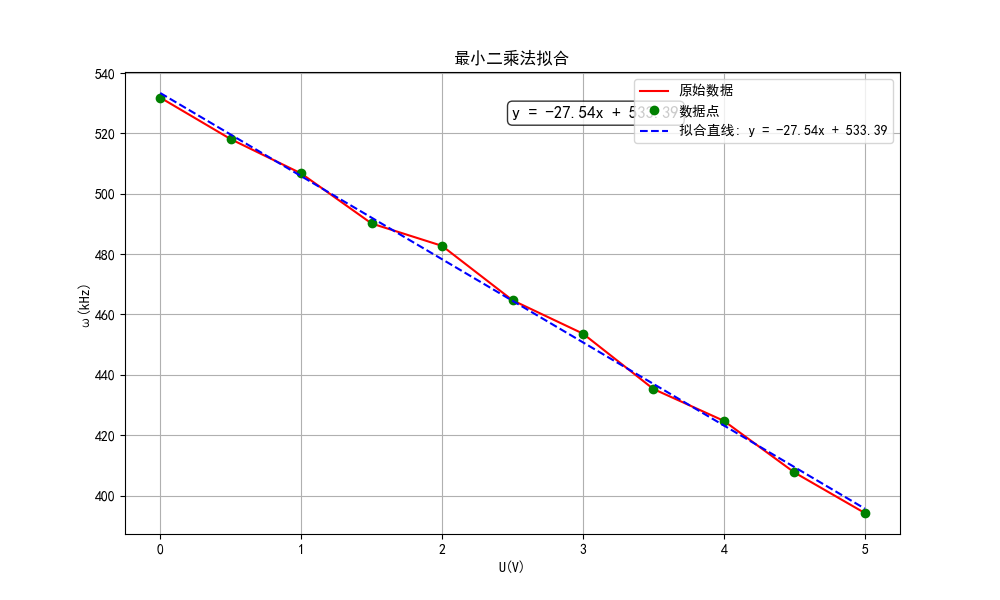
\includegraphics[width=0.7\linewidth]{picture_3}
     	\caption{}
     	\label{fig:picture3}
     \end{figure}
     
     \section{表5}
     \begin{tabular}{ccccc}
     	\toprule
     	\multicolumn{2}{c}{基带信号} & \multicolumn{3}{c}{光纤传输后解调的基带信号} \\
     	\cmidrule(lr){2-3} \cmidrule(lr){4-5}
     	幅度(V) & 频率(kHz) & 幅度(V) & 频率(kHz) & 信号失真度\\
     	\midrule
     	1.51& 8.00 & 0.152 & 8.00 & 不失真 \\
     	1.51& 4.00 & 0.152 & 4.00 & 不失真 \\
     	1.00& 8.00 & 0.1   & 8.00 & 不失真 \\
     	3.00& 8.00 & 0.188 & 8.00 & 失真 \\
     	\bottomrule
     \end{tabular}
\end{document}